\documentclass[10pt,a4paper]{article}
\usepackage[utf8x]{inputenc}
\usepackage{ucs}
\usepackage{amsmath}
\usepackage{amsfonts}
\usepackage{amssymb}
\usepackage{fullpage}
\usepackage{graphicx}
\usepackage{multirow}
\usepackage{url}
\author{Tobias Eriksson, Sebastian Sjögren}
\title{Gravitational N-body Simulation}
\begin{document}
\maketitle

\tableofcontents

\listoffigures

\listoftables

\newpage

\section{Introduction}
The goal of this project has been to implement two different algorithms 
simulating gravitational N-body systems and then parallelize them. 
First, we implemented the direct-sum algorithm, that for each body in the system
computes the gravitational force it exerts on every other body. 
The algorithm has a time complexity of $O(n^2)$, rendering it slow for large systems.
The second algorithm implemented, the Barnes-Hut simulation, works entirely 
different and has time complexity $O(n\log n)$.
Using the concept of domain decomposition, parallelizing these algorithms has been fairly straightforward.
All four programs features optional graphical support that allows viewing of the simulation in real-time. The programs are implemented in C, using Posix Threads (or \textsf{pthreads}) for the parallelized versions. The implementation and testing was done on Ubuntu Linux. 

The purpose of the report is to provide a summary of algorithmic and implementational problems and their solutions and some analysis of results acquired during performance testing.
\section{Programs}
This section gives a summary of each program implemented, and discusses solutions to some of the implementational problems that arose. The code itself is thoroughly documented, so for implementational details , please refer to the code.
\subsection{Sequential Direct-Sum}
The direct-sum is a straight-forward method. For each body in system, compute the gravitational forces exerted on every other body and update their positions in the system. While this method is relatively straightforward and easy to implement, the squared complexity makes it painfully slow to run when simulating large systems.

The algorithm iterates through the whole array of bodies, for a given number of times. For each unordered pair of bodies $i, j$, it computes the gravitational forces they exert on each other. When all forces are calculated, bodies are moved according to the resulting velocity vector, derived from the gravitational forces.
\subsection{Parallelized Direct-Sum}
To achieve some effectiveness on multicore systems, it advisable to try and parallelize the direct-sum algorithm. Forces are calculated iteratively over the array of bodies, which makes it possible to have a number of \emph{worker} threads to calculate the forces for a subset of bodies concurrently and in parallel. 

The most straightforward solution would be do distribute the for-loop over the array of bodies evenly between the worker threads. However, the workload for each worker would be unbalanced and unfair, since the inner for-loop iterates over a lesser and lesser number of bodies. Consider this situation: we have two worker threads \textsf{A} and \textsf{B}. Assuming that the number of bodies $n$ is even, then each worker would get $n/2$ bodies to iterative over. Then worker \textsf{A} would in the first iteration calculate the forces body $i = 1$ exert on bodies $j = 2,..,n$ and vice versa. The second iteration would calculate the forces for $i = 2$ and $j = 3,..,n$ and so on. However, \textsf{B} would calculate the forces for $i = n/2$ and $j = n/2 +1,..,n$ then $i = n/2 + 1$ and $j = n/2 + 2,...,n$ and so on. It's clear that worker \textsf{A} will have to do much more work than \textsf{B}, and thus the solution is unfair.

To make workload distribution more fair, there's a method known as \emph{reverse stripes}\cite{mpd}. The idea is that the body each worker works with alternates, in a $striped$ pattern. If we have two workers \textsf{A} and \textsf{B}, the bodies will be given to the workers in the pattern $(\textsf{A}, 0)$, $(\textsf{B}, 1)$, $(\textsf{B}, 2)$, $(\textsf{A}, 3)$ $(\textsf{A}, 4)$, $(\textsf{B}, 5)$ and so on. 

There are two main points of concern regarding synchronization. The first is that no worker is allowed to either move bodies until all forces are calculated or calculate new forces until all bodies have been moved. This is easily solved with barriers (see figure 1).

\begin{figure}[h!]
\begin{verbatim}
for(i = 0; i < num_steps; ++i) {
    compute_forces(id);
    barrier();   
    compute_positions(id);
    barrier();
}
\end{verbatim}
\caption{Solving the first synchronization problem with barriers}
\end{figure}
The second point of concern pertains mutual exclusion while updating of force vectors. Consider the sequential direct-sum solution. In it, for each unordered pair of bodies $i, j$, both their forces are computed. That's fine since the program is sequential, but in parallel it becomes a problem. It's highly probable that more than one worker makes changes to body $i$'s force vector concurrently, making the task a critical section. 

This is solved using a matrix of force vectors -- rather than assign one force vector per body there's a force vector \textit{matrix} of dimension num\_threads $\times$ num\_bodies. There's one partial force for each body per worker thread meaning this task is no longer a critical section. Later, when calculating new positions for bodies, these partial force vectors are simply summed up, used in computations and then reset for next iteration.
\subsection{Sequential Barnes-Hut}
The Barnes-Hut algorithm differs completely from the direct-sum algorithm. The main idea behind the algorithm is to group nearby bodies and approximate them as one single body. If such a group is sufficiently far away from concerned body, its gravitational can be approximated using its center of mass, which is the average position of a body in that group weighted by their mass\cite{princeton}.

The algorithm recursively divides the set of bodies into groups by storing them in a quad-tree. A quad-tree is similar to a binary tree, but each node has a maximum of four children instead of two. Each node in the tree represents a square region in two dimensional space, and each of it's children represents the quadrants of that square. The space is recursively divided into quadrants until each subdivision contains zero or one bodies. Each leaf node represents a single body and each internal node represents the group of bodies beneath it and holds the center of mass and total mass for it. See figure 2 for a graphical example with 8 bodies.

\begin{figure}[h!]
\centering 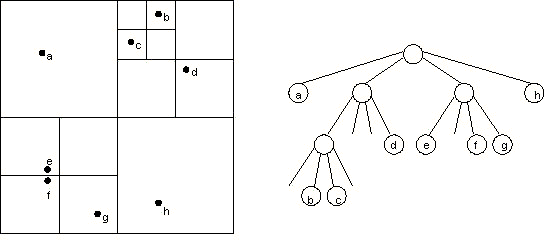
\includegraphics[scale=0.5]{images/bhtree}
\caption{8 bodies divided a quad-tree\cite{princeton}.}
\end{figure}

Forces exerted on bodies are calculated by traversing the nodes of the tree starting, always starting from the root. If the center-of-mass of an internal node is sufficiently far from concerned body, the force is calculated using the center-of-mass and total mass, as if it were a single body. If the internal node isn't far away enough, recursively traverse each of its subtrees. To find a criteria for evaluating whether a node is sufficiently far away, the quotient $s/d$ is computed, where s is the width of the region of that nodes, and d is the distance between the concerned body and the node's center-of-mass. This quotient is compared to some threshold value $\theta$, that can be given as a parameter on the command line. By adjusting this threshold, one can change the speed and accuracy of the simulation, $\theta = 0$ beeing the most accurate setting, as it will cause the algorithm never to approximate anything. A value commonly used is $\theta = 0.5$\cite{princeton}. 

\subsection{Parallized Barnes-Hut}
Even though the Barnes-Hut is effective, by parallelizing it, it can be made even more effective on multicore systems. The bodies are evenly distributed amongst the worker threads. One particular worker is responsible for rebuilding the quad-tree, as we didn't come up with any reasonably effective method to parallelize this task. Each worker is given a range of bodies for which it will calculate forces and positions, in a manner similar to the direct-sum algorithm.

As before, barriers  are needed to synchronize tasks. The first barrier is used to make workers wait for quad-tree to be built. The second and the third are used just like in the direct-sum method, to wait for the force computation and the position updating steps to be complete. In contrast to the direct-sum algorithm, each work is entirely disjoint, and there is no need for mutual exclusion when performing them.

\section{Evaluation}
To compare the different programs, a set of timing experiments were done. First, the number of steps to be used was chosen. Running the sequential direct-sum program for \textbf{37500} steps resulted in a running time of approximately 15 seconds, which is a sufficiently large reference value. Table 1 shows the simulation times for the different programs.
\begin{table}[h!]
\centering
\begin{tabular}{|l|l|l|l|l|l|}
\hline
Program & Bodies & 1 worker & 2 workers & 3 workers & 4 workers\\ \hline
\multirow{3}{*}{Seq. Direct-Sum} & 120 &  15.1 s & - & - & -\\
 & 180 & 33.6 s & - & - & - \\
 & 240 & 59.7 s & - & - & - \\ \hline
 \multirow{3}{*}{Par. Direct-Sum} & 120 &  15.8 s &  8.79 s &  7.36 s & 5.9 s\\
 & 180 & 35.9 s & 18.3 s & 12.8 s & 12.7 s\\
 & 240 & 63.4 s & 33.0 s & 22.4 s & 17.2 s\\ \hline
 \multirow{3}{*}{Seq. Barnes-Hut} & 120 & 25.5 s & - & - & -\\
 & 180 & 39.4 s & - & - & -\\
 & 240 & 55.5 s & - & - & -\\ \hline
 \multirow{3}{*}{Par. Barnes-Hut} & 120 & 20.4 s & 12.3 s & 13.9 s & 12.4 s\\
 & 180 & 33.7 s & 22.6 s & 22.3 s & 19.6 s\\
 & 240 & 55.3 s & 36.1 s & 30.6 s & 26.4 s\\ \hline
\end{tabular}
\caption{Median running times for the different programs.}
\end{table}
Results in Table 1 are median times of 5 test runs for each program, bodies and number of threads (if applicable). The programs were executed on a KTH Workstation, with 4 cores at clock speed 2.83 GHz. The results are, all in all pretty much expected. Figure 3 shows the speedups of the different programs with various parameters.

\begin{figure}[h!]
\centering 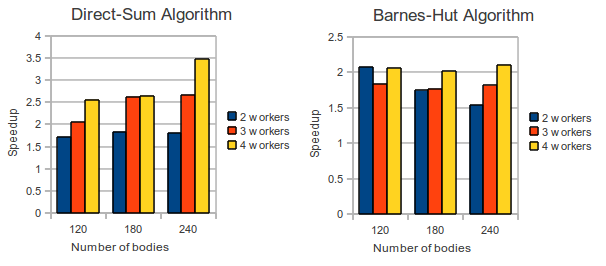
\includegraphics[scale=0.75]{images/speedup-graphs}
\caption{Speedups for the different programs with various parameters.}
\end{figure}

For the \textbf{Seq. Direct-Sum} program, a 50\% increase in bodies seems to result in a doubling of running time. This is expected because of the $O(n^2)$ time complexity. 

This is true for \textbf{Par Direct-Sum} as well, when using only 1 worker thread. Although, when running it with 2 threads, the running time is almost halved, which proves the parallization was successfully implemented. Running time continue to drop as we move on with 3 and 4 worker threads.

The \textbf{Seq. Barnes-Hut} program runs for almost twice as long time as Seq. Direct-Sum. This seems odd at first, but considering that the Barnes-Hut algorithm claims a lot more overhead (primarly memory allocation, extensive and repeated use of \textsf{malloc()}, it isn't very suprising. We did a small test with 2000 bodies and 300 steps, which the Seq. Barnes-Hut completed in about 3 seconds, but Seq. Direct-Sum took over half a minute to finish.

The results for the \textbf{Par. Barnes-Hut} are somewhat misleading partly due to the previously named overhead but mainly because there's one single thread that's responsible for building the tree over and over for each iteration. If the number of bodies is small, as in these cases, the tree building task becomes very large in relation to the size of force and position computation tasks. Thus the program scales badly with respect to the increase of worker threads. Just to be sure of this, we performed an additional test concerning the parallelized Barnes-Hut program only. The results of running the program on different number of threads for \textbf{300} steps with \textbf{10000} bodies is seen in Table 2.
\begin{table}[h!]
\centering
\begin{tabular}{|l|r|r|r|r|}
\hline
Program & 1 worker & 2 workers & 3 workers & 4 workers\\ \hline
Par. Barnes-Hut & 15.5 s & 9.24 s & 7.47 s & 6.22 s \\ \hline
\end{tabular}
\caption{Median running times for parallelized Barnes-Hut program simulating a larger system}
As seen, speedup for Barnes-Hut reaches up to around 2.5 using 4 worker threads. The reason for not getting any better speedup than this is might be that one thread alone performs the tree building task, while the other workers have to wait.
\end{table}

\section{Conclusions}
Speedups for the parallelized direct-sum algorithm is clearly better than speedups of the Barnes-Hut algorithm. It's possible that, had we succeeded in parallelizing tree building as well, Barnes-Hut would have reached better speedups. Although we feel that the performance gain received comparing Barnes-Hut with direct-sum sort of make up for this. Using SDL/OpenGL graphics, a Barnes-Hut simulation of up to bodies runs smoothly at around 20-30 fps (estimate) on a decent system, while the direct-sum program has trouble producing more than around 30-40 images per minute using the same parameters. Also, when performance analysing the Barnes-Hut implementation using the profiling tool \textbf{gprof} it became clear that building the tree doesn't seem to be much of a bottle neck anyway, as an execution spends about 5-8\% of the time executing that code.

\begin{thebibliography}{9}
\bibitem{mpd}
	Gregory R. Andrews, 2000, \emph{Foundations of Multithreaded, Parallel, and Distributed Programming}
	Addison-Wesley.
\bibitem{princeton}
	Tom Ventimiglia and Kevin Wayne, 2003, \emph{Barnes-Hut Galaxy Simulator}, \url{http://www.cs.princeton.edu/courses/archive/fall03/cs126/assignments/barnes-hut.html}. Last retrieved \today.
	
\end{thebibliography}
\end{document}